\chapter{Background}
\label{ch:background}

This chapter reviews the background the renderer builds on. It moves from the general to the
specific: Monte~Carlo integration (the numerical method), the rendering equation and its
volumetric generalisation (the physics), the Gaussian kernel-mixture model (the scene
representation), and hardware-accelerated ray tracing (the platform it all runs on). A recurring theme, picked up
in earnest in \Cref{ch:architecture}, is that the Gaussian primitive is \emph{analytically
tractable}: integrals that are stochastic for a general medium have closed forms for a Gaussian.
Exploiting this separates the renderer from the segment-marching reference.

\section{Monte Carlo integration}
\label{sec:monte-carlo}

Most quantities in physically based rendering are integrals with no analytic solution. Monte~Carlo
(MC) integration estimates $\int_{\Omega} f(\bm{x})\,\mathrm{d}\bm{x}$ as a weighted average of the
integrand at random sample points $\bm{x}_i$ drawn from a probability density $p$:
\[
  \langle F \rangle = \frac{1}{n}\sum_{i=1}^{n} \frac{f(\bm{x}_i)}{p(\bm{x}_i)},
  \qquad \bm{x}_i \sim p .
\]
The estimator is unbiased for any $p$ whose support covers that of $f$: its expected value is
exactly the integral. Its error is random noise that averages out, rather than a systematic offset
that does not. Its variance falls as $O(1/n)$ (when $f/p$ has finite variance), so the error falls as $O(1/\sqrt{n})$ \emph{independently of
dimension}. This dimension-independence is why MC is the workhorse for the high-dimensional
transport integrals below, where deterministic quadrature is impractical.

\Cref{fig:mc-integ} makes both behaviours concrete on a one-dimensional example: a single running
estimate settles onto the true value inside its shrinking confidence band, and the RMS error across
independent runs falls along the $-\tfrac12$ slope. The constant in front of that $1/\sqrt{n}$ rate is
what every variance-reduction technique in this
thesis targets. \emph{Importance sampling}---choosing $p$ to resemble $f$---shrinks it, vanishing
entirely when $p \propto f$ (for non-negative $f$). Two consequences recur. First, because error scales as $1/\sqrt{n}$,
halving the noise costs four times the samples; constant-factor variance reductions are therefore
worth pursuing (\Cref{ch:optimization}). Second, replacing pseudo-random points with a
low-discrepancy sequence such as Sobol~\cite{Sobol1967} with Owen scrambling~\cite{Owen1998} can
improve the rate for smooth integrands---an option \Cref{ch:optimization} measures and ultimately
does not adopt.

\begin{figure}[htp]
  \centering
  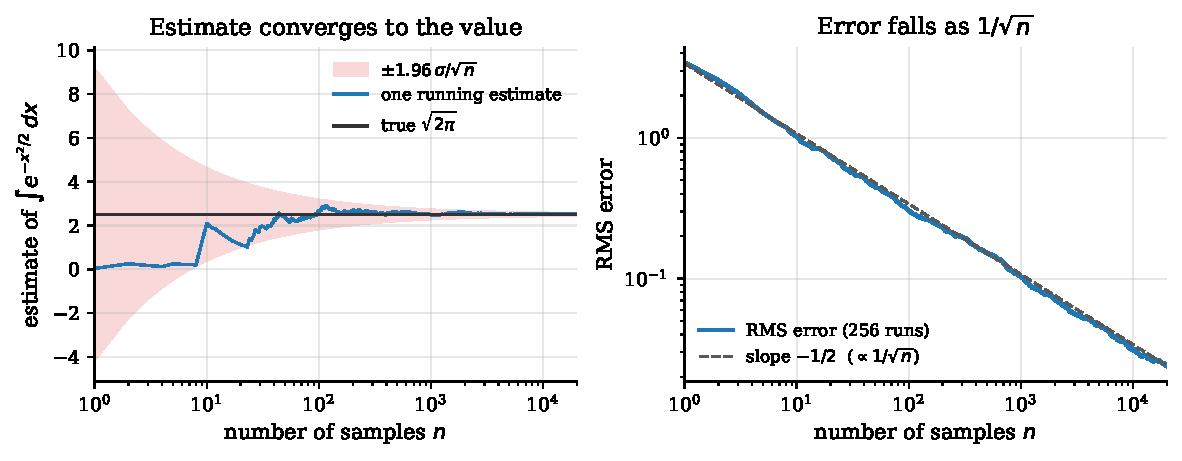
\includegraphics[width=\linewidth]{figures/mc_integ.pdf}
  \caption{Monte~Carlo integration of $f(x)=e^{-x^2/2}$ (true value $\sqrt{2\pi}$), estimated by the
sample mean of $f/p$ with $p$ uniform on $[-5,5]$. \emph{Left:} one running estimate settles
onto the true value inside the shrinking $\pm1.96\,\sigma/\sqrt{n}$ band---a \num{95}\,\%
confidence interval. \emph{Right:} the RMS error over \num{256} independent runs falls along
a slope-$(-1/2)$ line: error $\propto 1/\sqrt{n}$, so halving it costs four times the
samples. (An illustrative \texttt{numpy} experiment performed for this thesis; \num{256}
runs of $2\times10^4$ samples each.)}
  \label{fig:mc-integ}
\end{figure}

\section{The rendering equation}
\label{sec:rendering-equation}

Light transport at surfaces is governed by the rendering equation~\cite{Kajiya1986}, which expresses the radiance---the flow of light along a ray: power per unit area per unit
solid angle, the quantity a pixel ultimately records---leaving a point $\bm{x}$ in
direction $\bm{\omega}_o$ as emitted radiance
plus reflected incident radiance integrated over the hemisphere $\Omega$:
\[
  L_o(\bm{x},\bm{\omega}_o) = L_e(\bm{x},\bm{\omega}_o) +
  \int_{\Omega} f_r(\bm{x},\bm{\omega}_i,\bm{\omega}_o)\,
  L_i(\bm{x},\bm{\omega}_i)\,\lvert \bm{n}\cdot\bm{\omega}_i\rvert \,\mathrm{d}\bm{\omega}_i ,
\]
where $f_r$ is the bidirectional reflectance distribution function (BRDF) and $\bm{n}$ the surface normal.
The integral is estimated by MC: sample incident directions, evaluate, recurse.
\emph{Path tracing} applies this recursion along light paths from the camera, accumulating
contributions until paths are terminated by Russian roulette~\cite{ArvoKirk1990}. Roulette randomly ends
low-contribution paths and reweights the survivors, trading variance for speed without introducing bias. The media this
thesis renders, however, interact with light not at surfaces but throughout their interior; the
next section gives the volumetric form of the same physics.

\section{Volumetric light transport}
\label{sec:volumetric-light-transport}

Whereas the surface rendering equation describes light that scatters at well-defined interfaces,
the media this thesis renders---clouds, smoke, and other participating volumes---interact with
light \emph{throughout} their extent. The governing model is the \emph{radiative transfer
equation}~\cite{Chandrasekhar1960}, whose Monte~Carlo treatment for rendering is surveyed by
Nov\'ak et al.~\cite{Novak2018}. This section collects the volumetric quantities the renderer is built
on: optical depth and transmittance, free-flight distance sampling, the phase function, and the
variance-reduction tools (next-event estimation and multiple importance sampling) that the later
chapters extend.

\subsection{Optical depth and transmittance}

A ray $\bm{r}(t)=\bm{o}+t\bm{d}$ crossing a medium with extinction coefficient $\sigma_t(\bm{x})$---the probability, per
unit length of travel, that light interacts with the medium---is attenuated according to
the Beer--Lambert law. The fraction of radiance
surviving from $0$ to $t$ is the \emph{transmittance}
\[
  T(t) = \exp\!\big(-\tau(t)\big), \qquad
  \tau(t) = \int_0^{t} \sigma_t\big(\bm{r}(s)\big)\,\mathrm{d}s,
\]
where $\tau(t)$ is the \emph{optical depth} accumulated along the segment. For a general
heterogeneous medium $\tau$ has no closed form; instead, free flights are sampled and transmittance
$T = e^{-\tau}$ estimated stochastically---for instance by delta tracking~\cite{Woodcock1965} or its
decomposition variants~\cite{Kutz2017}. One property of the Gaussian kernel-mixture representation
is exploited throughout this work: a single Gaussian primitive's contribution to $\tau$ \emph{does}
admit a closed form in terms of the error function (\Cref{sec:kernel-mixture}). The per-primitive optical depth is therefore analytic rather than sampled.

Extinction is the sum of two loss channels, absorption and scattering:
$\sigma_t = \sigma_a + \sigma_s$. The \emph{single-scattering albedo}
$\alpha = \sigma_s/\sigma_t$ is the fraction of extinguished light that is scattered
onward rather than absorbed; at each scattering event a path's carried energy is
multiplied by $\alpha$. Albedo $0$ is thus a purely absorbing medium
(\Cref{sec:absorption-ladder}), albedo $1$ a purely scattering one (the furnace test of
\Cref{sec:scattering-ladder}), and the production media in this thesis use albedo $0.9$.

\subsection{Free-flight sampling}

Path tracing a volume requires sampling the distance $t$ to the next scattering event in proportion
to the collision density $\sigma_t(\bm{r}(t))\,T(t)$. Equivalently, $t$ is drawn so that the
accumulated optical depth reaches an exponentially distributed target: given $\xi\sim\mathcal{U}[0,1)$,
one solves
\[
  \tau(t) = -\ln(1-\xi)
\]
for $t$, the \emph{free-flight} distance. In a heterogeneous medium this is solved implicitly by
tracking---there is no closed form for $\tau^{-1}$---and the reference implementation marches the ray
segment by segment and root-finds $t$. Because each Gaussian primitive here has an analytic,
invertible optical-depth profile, its free-flight distance can instead be sampled in \emph{closed
form}. This property underlies the sort- and march-free scatter sampling introduced in
\Cref{ch:architecture}.

\subsection{The phase function}

At a scattering event the outgoing direction is drawn from the \emph{phase function}
$p(\bm{\omega}_i,\bm{\omega}_o)$, the volumetric analogue of the BRDF. This work uses the
Henyey--Greenstein model~\cite{HenyeyGreenstein1941},
\[
  p_{\mathrm{HG}}(\cos\theta) =
  \frac{1}{4\pi}\,\frac{1-g^{2}}{\big(1+g^{2}-2g\cos\theta\big)^{3/2}},
\]
whose single parameter $g\in(-1,1)$ controls anisotropy; $\theta$ is the angle between the incoming
and outgoing directions. Here $g>0$ is forward scattering (clouds are strongly forward, $g\approx 0.85$),
$g=0$ is isotropic (an idealisation, and the high-order multiple-scattering limit), and $g<0$ is
backscattering. $p_{\mathrm{HG}}$ is
cheap to importance-sample and integrates to one over the sphere, both properties the estimator
below relies on.

\subsection{Next-event estimation and multiple importance sampling}
\label{sec:nee-mis}

Letting a path find the light only by chance---sampling the phase function alone---is high variance
for small or distant emitters. \emph{Next-event estimation} (NEE) instead adds, at every scattering vertex (each
scattering event along the path), an explicit connection to a sampled light direction,
weighted by the transmittance along the \emph{shadow ray}: the straight ray traced from
the vertex toward the light to measure how much of it gets through. Phase-function sampling and NEE are each effective in complementary regimes, so they are
combined with \emph{multiple importance sampling} (MIS)~\cite{VeachGuibas1995}. A sample drawn from
strategy $s$ with density $p_s$ receives the balance-heuristic weight
\[
  w_s(\bm{x}) = \frac{n_s\,p_s(\bm{x})}{\sum_k n_k\,p_k(\bm{x})},
\]
where $n_s$ is the number of samples allocated to strategy $s$. This weighting trusts each strategy in
proportion to how likely it was to have produced the sample. Its variance is provably within a
small additive term of the best achievable combination of the given strategies.
\Cref{ch:optimization} revisits this direct-lighting estimator, replacing the light-sampling
strategy with resampled importance sampling~\cite{Talbot2005} while retaining the MIS scaffold.

\section{Gaussian kernel-mixture volumes}
\label{sec:kernel-mixture}

The scene representation this thesis renders is a \emph{Gaussian kernel mixture}
(\Cref{fig:gmms}): the medium's
extinction field is modelled as a weighted sum of $N$ Gaussian kernels, in general anisotropic,
\[
  \sigma_t(\bm{x}) = \sum_{k=1}^{N} w_k\,
  \mathcal{G}(\bm{x};\bm{\mu}_k,\Sigma_k),
  \qquad
  \mathcal{G}(\bm{x};\bm{\mu},\Sigma) =
  \exp\!\Big(-\tfrac{1}{2}(\bm{x}-\bm{\mu})^{\!\top}\Sigma^{-1}(\bm{x}-\bm{\mu})\Big),
\]
where each kernel has a mean $\bm{\mu}_k$ (its centre), a covariance $\Sigma_k$ (its anisotropic
extent and orientation), and a weight $w_k$ (a peak-extinction amplitude). \Cref{ch:architecture} works
with the equivalent mass-normalised form, in which the per-primitive $\sigma_t$ absorbs the
$(2\pi)^{-3/2}\prod_i s_i^{-1}$ normalisation. Such mixtures are fit to a reference
volume by expectation--maximisation or, in the radiance-field setting, by gradient descent against
images. The primitives are the same anisotropic 3D Gaussians popularised by 3D Gaussian
Splatting~\cite{3DGS} and carried into volumetric ray tracing by Condor et
al.~\cite{DSYG} (\Cref{ch:related-work}). One convention, shared with the reference and
used silently throughout, should be stated here: although a Gaussian has infinite tails,
each primitive is truncated to a bounded \emph{support}---the ellipsoid at three standard
deviations ($3\sigma$) along each principal axis---outside which its density is taken as
exactly zero. Every later statement about a ray ``entering'' or ``leaving'' a primitive
refers to crossing this $3\sigma$ boundary, and the instanced unit sphere of
\Cref{sec:gpu-ray-tracing} is scaled to it.

One property makes this representation tractable for ray tracing: a single Gaussian's contribution
to the optical depth along a ray has a \emph{closed form}. Both the reference method~\cite{DSYG} and
this work depend on it. Restricting a 3D Gaussian to the line
$\bm{r}(t)=\bm{o}+t\bm{d}$ yields a one-dimensional Gaussian in $t$, and the integral of a Gaussian
is an error function. Hence the per-primitive optical depth
\[
  \tau_k(t) = \int_0^{t} w_k\,\mathcal{G}\big(\bm{r}(s);\bm{\mu}_k,\Sigma_k\big)\,\mathrm{d}s
\]
evaluates to a scaled difference of $\operatorname{erf}$ terms rather than a sampled estimate. This
analytic, invertible per-primitive optical depth is the property most heavily used in
\Cref{ch:architecture}. It lets each primitive's free-flight distance be drawn in closed
form, eliminating the segment marching and root-finding the reference requires.

\begin{figure}[htp]
  \centering
  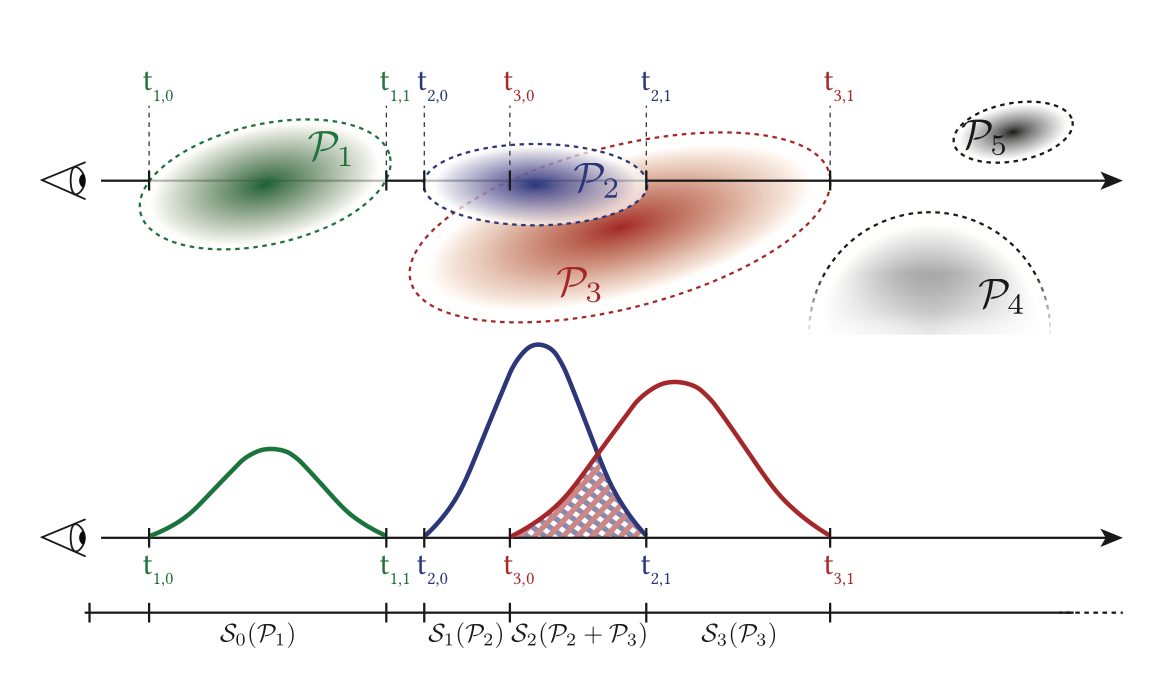
\includegraphics[width=11cm]{images/dsyg-gmms.png}
  \caption{A ray traversing a Gaussian kernel mixture. Each primitive's contribution to the optical
  depth along the ray---and the overlap region of primitives $\mathcal{P}_2$ and
  $\mathcal{P}_3$---is available in closed form, avoiding stochastic estimation of the extinction.
  Figure taken directly from Condor et al.~\cite{DSYG}.}
  \label{fig:gmms}
\end{figure}

Condor et al.~\cite{DSYG} additionally explore Epanechnikov
kernels~\cite{Epanechnikov1969}, which decay to exactly zero at
a finite radius rather than asymptotically. Compact support reduces the average number of primitives
overlapping a ray and packs more tightly into the ray-tracing acceleration structure
(\Cref{sec:gpu-ray-tracing}), which the reference reports
can improve reconstruction efficiency. This thesis retains the Gaussian kernel (\Cref{ch:optimization} notes where the choice
would matter). The \emph{forward} optical depth is closed-form for either kernel, but the argmin sampler
additionally needs a practical closed-form \emph{inverse}, which is Gaussian-specific. For the
Epanechnikov that inverse is impractical, and even the reference resorts to a numerical solver for a
single such kernel.

\section{Ray tracing on the GPU}
\label{sec:gpu-ray-tracing}

Rendering a kernel-mixture volume by ray tracing requires, for every camera ray, finding which
primitives it intersects and in what order. A ray is the half-line $\bm{r}(t)=\bm{o}+t\bm{d}$, and
testing it against a single bounded primitive is a cheap algebraic intersection; testing it against
all $N$ primitives in a scene is not. \emph{Acceleration structures} reduce this from $O(N)$ to a typical
$O(\log N)$ by pruning whole groups of primitives at once---the spatial analogue of a binary search.
The dominant choice is the bounding
volume hierarchy (BVH)~\cite{KayKajiya1986,MacDonaldBooth1990}, a tree of nested
bounding volumes in which a ray that misses a node misses everything beneath it.

Contemporary GPUs implement BVH traversal and ray--box/ray--primitive intersection in dedicated
hardware, exposed through programmable pipelines such as NVIDIA OptiX~\cite{Optix}. An OptiX pipeline
is assembled from user-supplied programs---ray generation, intersection, any-hit, closest-hit, and
miss---executed over a two-level acceleration structure. A geometry acceleration structure (GAS)
holds the primitives, instanced through an instance acceleration structure (IAS) with per-instance
transforms. This separation lets a scene of thousands of distinct ellipsoids be represented as
\emph{one} unit-sphere GAS instanced many times. Each instance carries the affine transform that
maps the unit sphere to a primitive's centre, scale, and orientation. \Cref{ch:architecture} builds
directly on these primitives. It uses the built-in sphere intersection over such a GAS/IAS and,
unconventionally, an any-hit program (rather than the conventional closest-hit, which
keeps only the nearest intersection and ends the query) to \emph{collect} all of a ray's
primitive entries in a single traversal. Together with the analytic optical depth of
\Cref{sec:kernel-mixture}, this collection is the basis of the design in \Cref{ch:architecture}.

Two facts about GPU execution recur in \Cref{ch:architecture,ch:optimization}. First, a
GPU runs threads in \emph{warps}: fixed groups of \num{32} that execute one common
instruction stream in lockstep, each thread occupying one \emph{lane}. When the threads of
a warp take different branches or wait on different memory---\emph{divergence}---some
lanes sit idle while the others proceed, and throughput falls in proportion. Second, the
hardware hides memory latency not with large caches but by keeping many warps resident and
switching among them every cycle; \emph{occupancy}---how many warps are resident relative
to the hardware maximum---therefore bounds how much latency can be hidden.
